\chapter{Ideen und Konzepte}

\section{Grundidee}
Für die Konzepte, welche im Kapitel \ref{ch:konzeptEins} und \ref{ch:konzeptZwei} beschrieben sind, ist die Ausgangslage, dass die Gefahr besteht, dass Exemplare im Hochregallager in falsche Behälter deplatziert werden. Weiter ist vonseiten des Kunden gewünscht, dass die Exemplare nicht nachgerüstet werden müssen (siehe Protokoll \ref{app:sec:protokollKickoff}). Aus diesem Grund gilt für beide Konzepte, dass lediglich die vorhandenen HF RFID Tags zur Verwendung stehen und keine weiteren alternative Ideen verwendet werden können.

Das in Kapitel \ref{ch:konzeptEins} vorgestellte Konzept hat zum Ziel, dass bereits deplatzierte Exemplare im Hochregallager wiedergefunden werden können. Dabei wird dargelegt, wie vorgegangen werden soll, um die Suche möglichst effizient durchzuführen. Hierzu wird berechnet, wie lange eine Suche mit nur einer Antenne dauert und wie diese Suche optimiert werden kann, indem mehrere Antennen eingesetzt werden.

Das in Kapitel \ref{ch:konzeptZwei} vorgestellt Konzept hat zum Ziel, dass Exemplare, welche vom Personal in einen falschen Behälter platziert werden, vor der Einlagerung erkannt und der Behälter im System entsprechend markiert wird. In diesem Konzept werden verschiedene Möglichkeiten dargelegt, wie eine solche Erkennung mit der Hilfe einer neuen Scanstation erreicht werden kann. Es wird schliesslich eine mögliche Lösung empfohlen.

\chapter{Konzept Eins: Suche}
\label{ch:konzeptEins}
\section{Strategie}
Um die Ausgangslage zu verbessern, können verschiedene Ansätzte gewählt werden. In diesem Konzept wird die Möglichkeit der Exemplarfindung im Hochregallager untersucht. Sollte ein bestimmtes Exemplar verloren gehen, soll diese automatisiert im Hochregallager wiedergefunden werden. Die so vereinfachte Wiederfindung soll der Speicherbibliothek zu einer erhöhten Sicherheit bezüglich der Einlagerung der Exemplare verhelfen. Es soll bewirkt werden, dass deplatzierte Exemplare ohne grösseren personellen Aufwand wiederbeschafft werden können.

\section{Ideenbeschreibung}
Momentan fährt der Roboter nur die im System hinterlegte Position des Behälters an. Diese Fahrt wird durch die Software des Logistiksystems mitsamt des Roboters gesteuert. Neu soll die Software dieses Herstellers so erweitert werden (Siehe \ref{sec:roboterSWAnpassung}), dass der Roboter einen vordefinierten Pfad abfährt mit einem speziellen RFID Lesebehälter/Suchbehälter (Siehe \ref{sec:behaelterMitRFID}) und dabei noch Aktionen ausführt, wie die temporäre Einlagerung dieses Behälters und Zwischenlagerung des Behälters, welcher sich an der eingelagerten Stelle befand.
Würde nun ein Buch, welches von einer Bibliothek oder einem anderen Kunden bestellt wurde, nicht im entsprechenden Behälter zu finden sein, soll neu der spezielle RFID Lese-/Suchbehälter in das Hochregallager geschickt werden.


Dabei gibt es zwei Unterschiedliche Suchmodi. Als Erstes würde der Roboter mit dem Lese-/Suchbehälter in alle Gassen geschickt, wo dieser durch jede Reihe nacheinander fährt. Dabei wird jeweils vom Lese-/Suchbehälter der Vordere Behälter nach dem fehlenden Exemplar abgesucht. So kann in einer Kurzer Zeit ca. 50\% des Lagers nach dem deplatzierten Exemplar abgesucht werden. Würde nach diesem Suchvorgang die Lokalisation des Exemplares nicht erfolgreich abgeschlossen werden, würde in der Nacht die zweite Suchfunktion starten, bei welcher der Lese-/Suchbehälter im Hochregallager in der Höhe jeden dritten Platz eines äusseren bereits abgesuchten Behälters für eine kurze Zeit tauscht. Während der Lese-/Suchbehälter am äusseren Platz ist sucht er im hinteren Behälter nach dem Exemplar sowie in den dem abgesuchten Behälter direkt Benachbarten Behältern.

\subsection{Anpassungen Lagerverwaltungssoftware}
\label{sec:roboterSWAnpassung}
Für die Software der Lagerverwaltung soll die Herstellerfirma dieser Software diese um eine Schnittelle erweitern, welche es ermöglicht dem Roboter über das Netzwerk neue Fahrpositionsdaten mitzuteilen, zu welchen er anschliessend fährt. Es soll dabei möglich sein dem Roboter zu sagen, ob er einen Behälter tauschen soll oder nur an die Position fahren soll. Zudem soll die momentane Position des Roboters über diese Schnittelle abgefragt werden können. 

\subsection{Behälter mit RFID Ausrüstung}
\label{sec:behaelterMitRFID}
Die heutige RFID HF Technologie, welche bereits in der Speicherbibliothek zum Einsatz kommt ist auf ca. 1m Distanz beschränkt. Dies bedeutet, dass es nicht möglich ist alle Tags direkt vom Roboter aus zu lesen. Um alle Behälter auslesen zu können muss also der Behälter die Position eines anderen Behälters einnehmen, um den hinteren Behälter lesen zu können. Da es jedoch enorm zeitintensiv ist, jede vordere Kiste mit dem Lese-/Suchbehälter auszutauschen, sollen multiple Antennen zum Einsatzt kommen. Diese sollen so ausgerichtet werden, dass nicht nur der hintere Behälter sondern auch dessen Nachbarn ausgelesen werden können.
Die Antennen sollen gemäss Abbildung \ref{fig:antennenPositionen} ausgerichtet werden.

\begin{figure}[htb]
	\centering
	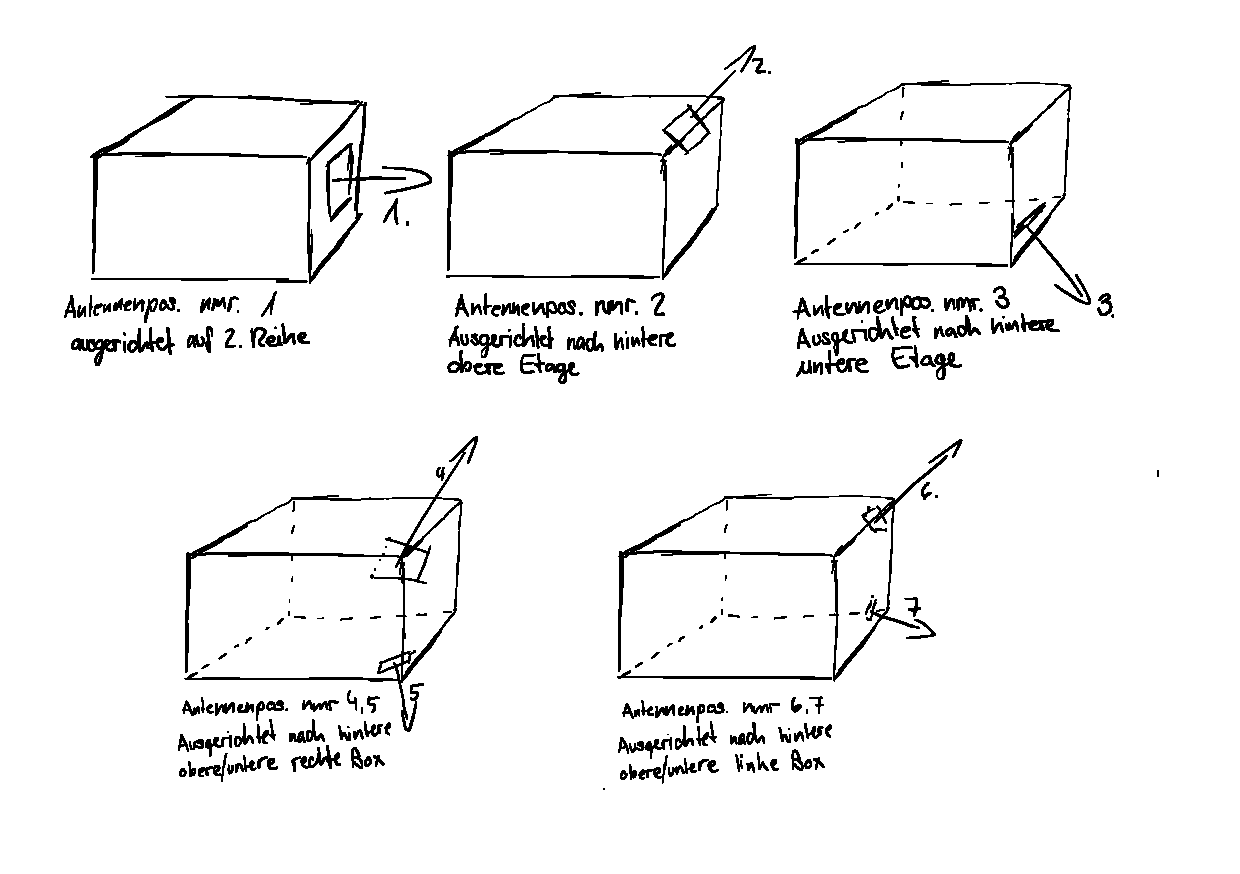
\includegraphics[keepaspectratio, width=1\textwidth]{antennen_auf_behaelter}
	\caption{Alle Antennenpositionen in einer Box für die Rechte Seite}
	\label{fig:antennenPositionen}
\end{figure}

In der Abbildung \ref{fig:distanzcalc} wird dargestellt, dass alle äusseren Behälter noch innerhalb der von HF RFID möglichen Lesedistanz von unter 1m liegen.

\begin{figure}[htb]
	\centering
	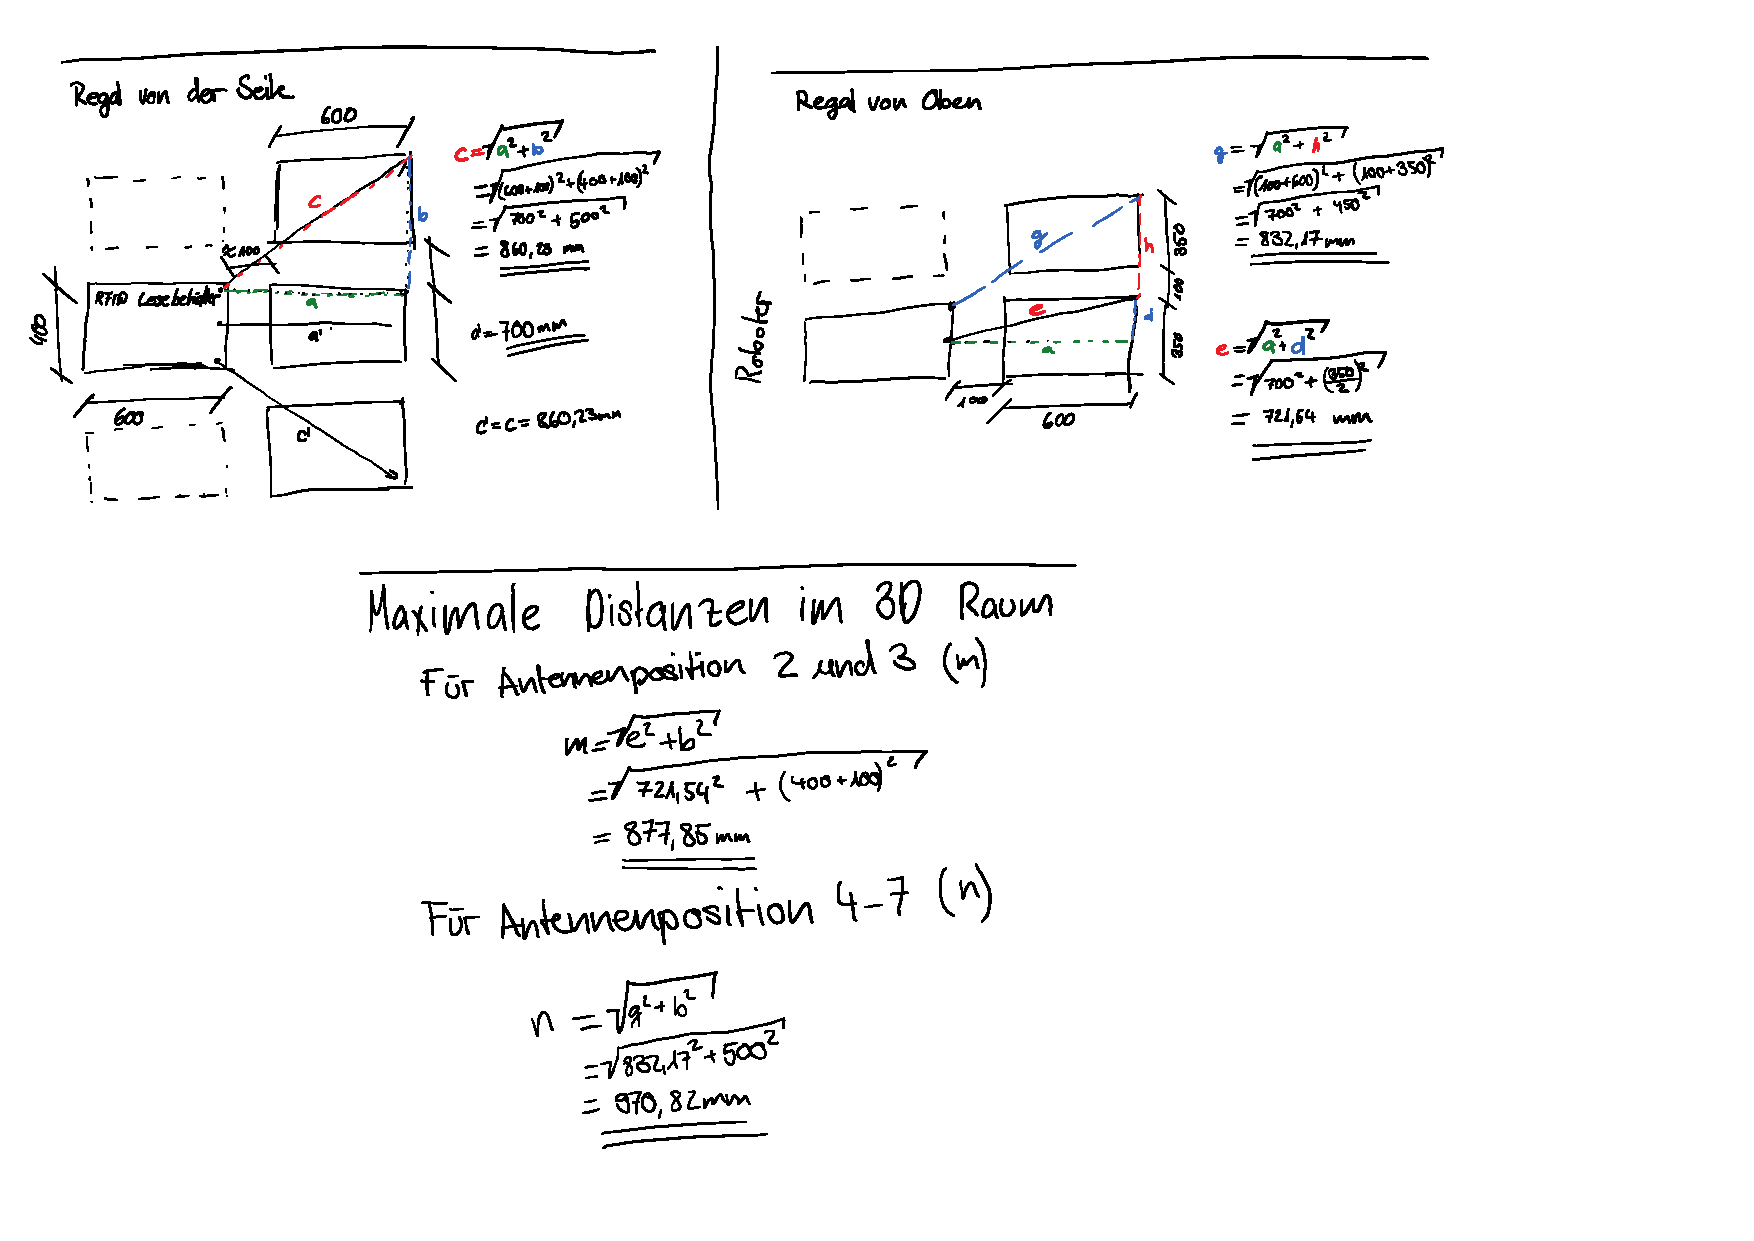
\includegraphics[keepaspectratio, width=1.2\textwidth]{berechnung_maximaler_distanz}
	\caption{Berechnung der maximalen Distanzen (alle Angaben in mm)}
	\label{fig:distanzcalc}
\end{figure}

Mangels Hersteller von RFID Lesegeräten, welche eine Lesereichweite von 1m oder mehr aufweisen, sollen folgende Komponenten von Feig Electronic verwendet werden. 
\begin{itemize}
	\item RFID Leser ID ISC.LR2500-A
	\item RFID Antennen ID ISC.ANT800/600
	\item RFID Antennenkabel ID ISC.ANT.C-A
	\item RFID 8xMultiplexer ID ISC.ANT.MUX
	\item Netzteil ID NET.24V-B
	\item Stromkabel ID CAB.NET.24V-B-EU
\end{itemize}

\clearpage
\subsection{Computer im Behälter}
Das RFID Lesegerät soll über einen kleinen, sich im Behälter befindenden Mini-Computer gesteuert werden. Dieser Computer soll über das bestehende WLAN Netzwerk auf die Datenbank zugreifen um die von RFID gescannten Behälter anhand der momentanen Position zu Identifizieren.  
Zudem soll die Fahrt des Roboter von diesem Minicomputer mittels den Anpassungen aus Kapitel  \ref{sec:roboterSWAnpassung} indirekt gesteuert werden.

Um diese Aufgabe zu übernehmen, soll ein Raspberry Pi verwendet werden.

\subsection{Kommunikation zum User}
Der User soll auf einem Stationären Computer über wichtige Informationen wie etwa die Dauer, den Fortschritt oder ob das zu suchende Exemplar bereits gefunden wurde informiert werden. Stationär bedeutet hier, dass es sich nicht um den Computer, welcher im Behälter ist, handelt.

\subsection{Stromzufuhr}
Für die komplette Stromversorgung soll ein Akku in dem Behälter verbaut werden, welcher genügend Kapazität für einen zehnstündigen Betrieb aufweist.

Der Stromverbrauch des RFID Lesers beträgt 35W bei 24V, das entspricht 1'458.32 mAh.
Der Stromverbrauch des Raspberry PI beträgt 4W bei 5V, das entspricht 800mAh.
Daher wird für eine Betriebsdauer von einer Stunde ein Akku mit einer Kapazität von mindestens 2'258.32 mAh benötigt. Um eine Betriebsdauer von zehn Stunden zu gewährleisten, benötigt der Akku eine Gesamtkapazität von mindestens 22'583.32 mAh.
Weiter hat er noch folgende Anforderungen.

\begin{itemize}
	\item USB Anschluss
	\item CH Wechselstromanschluss
	\item Geringes Gewicht
\end{itemize}

\subsection{Übersicht der Hardwarekomponenten}
Es sollen folgende Komponenten verwendet werden:

\begin{itemize}
	\item RFID Leser ID ISC.LR2500-A  (Feig)
	\item RFID Antennen ID ISC.ANT800/600 (Feig)
	\item RFID Antennenkabel ID ISC.ANT.C-A (Feig)
	\item Netzteil für Leser ID NET.24V-B (Feig)
	\item Netzkabel für Netzteil ID CAB.NET.24V-B-EU  (Feig)
	\item Minicomputer Raspberry PI 3 Model B + (Raspberry PI)
	\item USB-Kabel für Minicomputer Aukey CB-D11 (Aukey)
	\item Akku Goal Zero Yeti 400 Lithium (Goal Zero)
\end{itemize}

\section{Finanzierungsplan}

\subsection{Kosten}

\subsubsection{Lese-/Suchbehälter}
Die Einzelpreise von Feig sind gleichwertig zu einer Bestellung eines 100er Stapels und wurden von Euro in Schweizer Franken umgerechnet (Wechselkurs 1.14).

\begin{tabularx}{\textwidth}{|r|X|r|r|}
	\hline 
	\textbf{Menge} & \textbf{Produkt} & \textbf{Kosten(CHF)} & \textbf{Kosten gesamt(CHF)} \\
	\hline 
	1 & RFID Reader ID ISC.LR2500-A (Feig) & 1'200 & 1'200 \\ 
	\hline 
	2 & RFID Multiplexer 8-fach HF Multiplexer (Feig) & 500 & 1'000 \\ 
	\hline 
	14 & RFID Antennen ID ISC.ANT800/600 (Feig)& 760 & 10'640 \\
	\hline
	16 & RFID Antennenkabel ID ISC.ANT.C-A (Feig) & 20 & 320 \\
	\hline
	1 & Netzteil ID NET.24V-B (Feig) & 30 & 30 \\
	\hline
	1 & Netzkabel ID CAB.NET.24V-B-EU (Feig) & 4 & 4 \\
	\hline
	1 & Rapberry PI 3 Model B+ & 40 & 40 \\
	\hline
	1 & SB-Kabel für Minicomputer Aukey CB-D11 (Aukey) & 15 & 15 \\
	\hline
	1 & Akku Goal Zero Yeti 400 Lithium (Goal Zero) & 1'000 & 1'000 \\
	\hline
	1 & Behälter 986417 (Kaiserkraft) & 39 & 39 \\
	\hline
	& & & \textbf{14'288} \\
	\hline
\end{tabularx} 
\subsubsection{Umbau Roboter SW}
Basierend auf den Stundenkosten der Firma bbv Software Services AG wurde die folgende Approximation errechnet.
Die Stunden für die Umsetzung basieren auf Annahmen.

\begin{tabularx}{\textwidth}{|r|r|X|r|}
	\hline 
	\textbf{Stunden(h)} & \textbf{Lohn(CHF/h)} & \textbf{Beschrieb} & \textbf{Kosten gesamt(CHF)} \\
	\hline 
	50 & 180 & Umsetzung, sofern die Software die Befehle bereits über das Netztwerk entgegennimmt. & 9'000 \\
	\hline
	200 & 180 & Umsetzung, sofern die Software komplexere Anpassung benötigt & 36'000 \\
	\hline
	8 & 200 & Allgemeine RE und weitere Kosten & 1'600 \\
	\hline	
	& & & \textbf{10'600 bis 37'600} \\ 
	\hline
\end{tabularx}
\\
Die Gesamtkosten können also zwischen 10'600.- und 37'600.- schwanken. Wobei diese Werte auf zwei Approximationen beruhen, und somit für deren Einhalt nicht garantiert werden kann.

\subsubsection{Gesamt Rechnung}
\begin{tabularx}{\textwidth}{|X|r|}
	\hline
	\textbf{Beschreibung} & \textbf{Kosten (CHF)} \\
	\hline
	RFID Lese-/Suchbehälter & 14'288 \\
	\hline
	Umbau Roboter SW & 10'600 bis 37'600 \\
	\hline
	Weitere BDA für Implementation & 1'000 \\
	\hline
	& \textbf{25'888 bis 52'888} \\
	\hline
\end{tabularx}

\subsection{Kosten Manuelle Suche}
Würde ein Exemplar deplatziert werden, würde eine aufwendige Suche beginnen, welche bei etwa drei Millionen Exemplaren viel Zeit benötigt. Würde es theoretisch möglich sein ein Exemplar pro Sekunde zu durchsuchen bräuchte man etwa drei Millionen Sekunden. Dies entspricht 50'000 Minuten oder 833.32 Stunden oder 104.17 Arbeitstage à 8h oder knapp 5 Monaten. Würde diese Arbeit von einer Student*in mit einem Stundenlohn von etwa 20 CHF durchgeführt, könnte diese Suche bis zu 16'666.67 CHF kosten. Würde die Suche von einem Arbeiter der Speicherbibliothek übernommen werden, würden die Kosten noch höher ausfallen.

Die Kosten von 52'888 würden nach gut drei Suchvorgängen die Kosten der manuellen Suche eingeholt haben. Zusätzliche gäbe es einen Zeitgewinn von knapp 103 Arbeitstagen, da die Suche der Exemplare nach einem Tag abgeschlossen ist.


\chapter{Konzept Zwei: Prozessoptimierung}
\label{ch:konzeptZwei}

\section{Strategie}
Sollte ein Exemplar verlegt werden, soll dieses vor Einlagerung des betroffenen Behälters bemerkt werden und dieser aus dem Einlagerungsprozess aussortiert oder markiert werden. Die so behobene Möglichkeit eines Einlagerns eines falsch befüllten Behälters führt zu einem erhöhten Vertrauen in den Prozess. Das Verlegen eines Exemplars soll so verunmöglicht werden. Dies führt zu besserem Vertrauen der Mitarbeiter der Speicherbibliothek in den Prozess und bessere Möglichkeit für den Fokus auf die Hauptarbeitstätigkeit (nicht Kontrolle eines Behälters).

\section{Ideenbeschreibung}

Die generelle Idee dieses Konzepts ist eine Station in das Förderband zu integrieren, an der der Behälter durchfährt und an der Stelle dieser gescannt wird und Unstimmigkeiten erkannt werden. Dafür würden verschiedene Orte und Komponenten in Frage kommen. Diese sind daher jeweils einzeln in Betracht gezogen worden.

\subsection{Position}

\begin{figure}[htb]
	\centering
	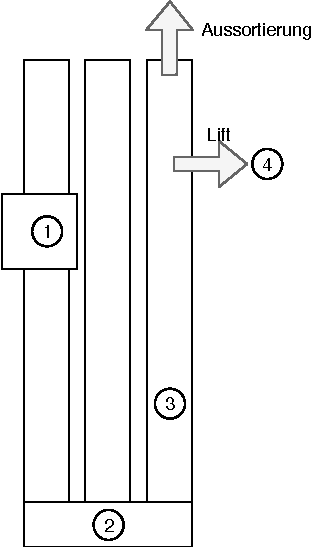
\includegraphics[keepaspectratio]{Position_Geraet}
	\caption{Mögliche Positionen des Geräts am Förderband}
\end{figure}

\subsubsection{Rüstplatz}
Da der Behälter während dem Entnehmen und Abfüllen des Behälters vergleichsweise lang stillsteht, hätte man an dieser Stelle sicher genug Zeit alle RFID Tags auszulesen. Mögliche Nachteile sind Platzmangel und Interferenzen durch Exemplare welche nicht im Behälter sind aber fälschlicherweise auch erfasst werden, da sie in der Nähe liegen.
\begin{itemize}
	\pro Genügend Zeit für das Auslesen aller Tags
	\pro Früh im Prozess für eine Meldung
	\con Interferenzen durch RFID markierte Exemplare in der Nähe
	\item Eventuell kein Platz für Antennen
	\item Eventuell Abschirmung/Justierung der Antennen möglich, sodass nur Exemplare im Behälter ausgelesen werden
\end{itemize}

\subsubsection{In einer Eckpartie}
Der Behälter führt auf dem Band zwei Rechtsdrehungen für einen Gesamtwinkel von \SI{180}{\degree} durch. An diesem Punkt bleibt der Behälter verhältnismässig lange in einem Bereich welcher von der Antenne abgedeckt werden sollte. Weiter befinden sich an dieser Position keine andere Exemplare oder Messstationen in der Nähe, was Interferenz verunmöglichen sollte.
\begin{itemize}
	\pro \textasciitilde\ drei Sekunden für das Auslesen der Tags zur Verfügung
	\pro Keine Interferenzen zu erwarten
	\con Nur beschränktes Zeitfenster
	\con Behälter in Bewegung
\end{itemize}

\subsubsection{Waage}
Der Behälter wird zur Bestimmung von Übergewicht gewogen, an dieser Stelle bleibt dieser etwa eine Sekunde an Ort und Stelle.
\begin{itemize}
	\pro Behälter bleibt an Ort und Stelle
	\pro Keine Interferenzen zu erwarten
	\con Nur beschränktes Zeitfenster
	\con Antenne kann nicht beliebig montiert werden
\end{itemize}

\subsubsection{Lift}
Der Behälter fährt vor Übergabe in das Hochregallager in einem Lift vertikal nach unten. Während dieser Zeit bleibt er längere Zeit still.
\begin{itemize}
	\pro Behälter bleibt an Ort und Stelle
	\pro Grosses Zeitfenster
	\con Beschränkter Platz da Lift
	\con Spät im Prozess
	\item Eventuell Interferenzen durch Liftmotoren
	\item Aussortierung eventuell nicht möglich
\end{itemize}

\subsection{Identifikation der RFID Tags}

\subsubsection{Eine Antenne}
\begin{itemize}
	\pro Keine Interferenzen
	\con Ausrichtung der Chips relevant
\end{itemize}

\subsubsection{Mehrere Antennen}
\begin{itemize}
	\pro Ausrichtung der Chips kann entgegengewirkt werden
	\pro Grössere Abdeckung
	\con Gegenseitige Interferenz
	\con Teurere Geräte nötig
	\con Mehr Platz wird benötigt
\end{itemize}

\begin{figure}[htb]
	\centering
	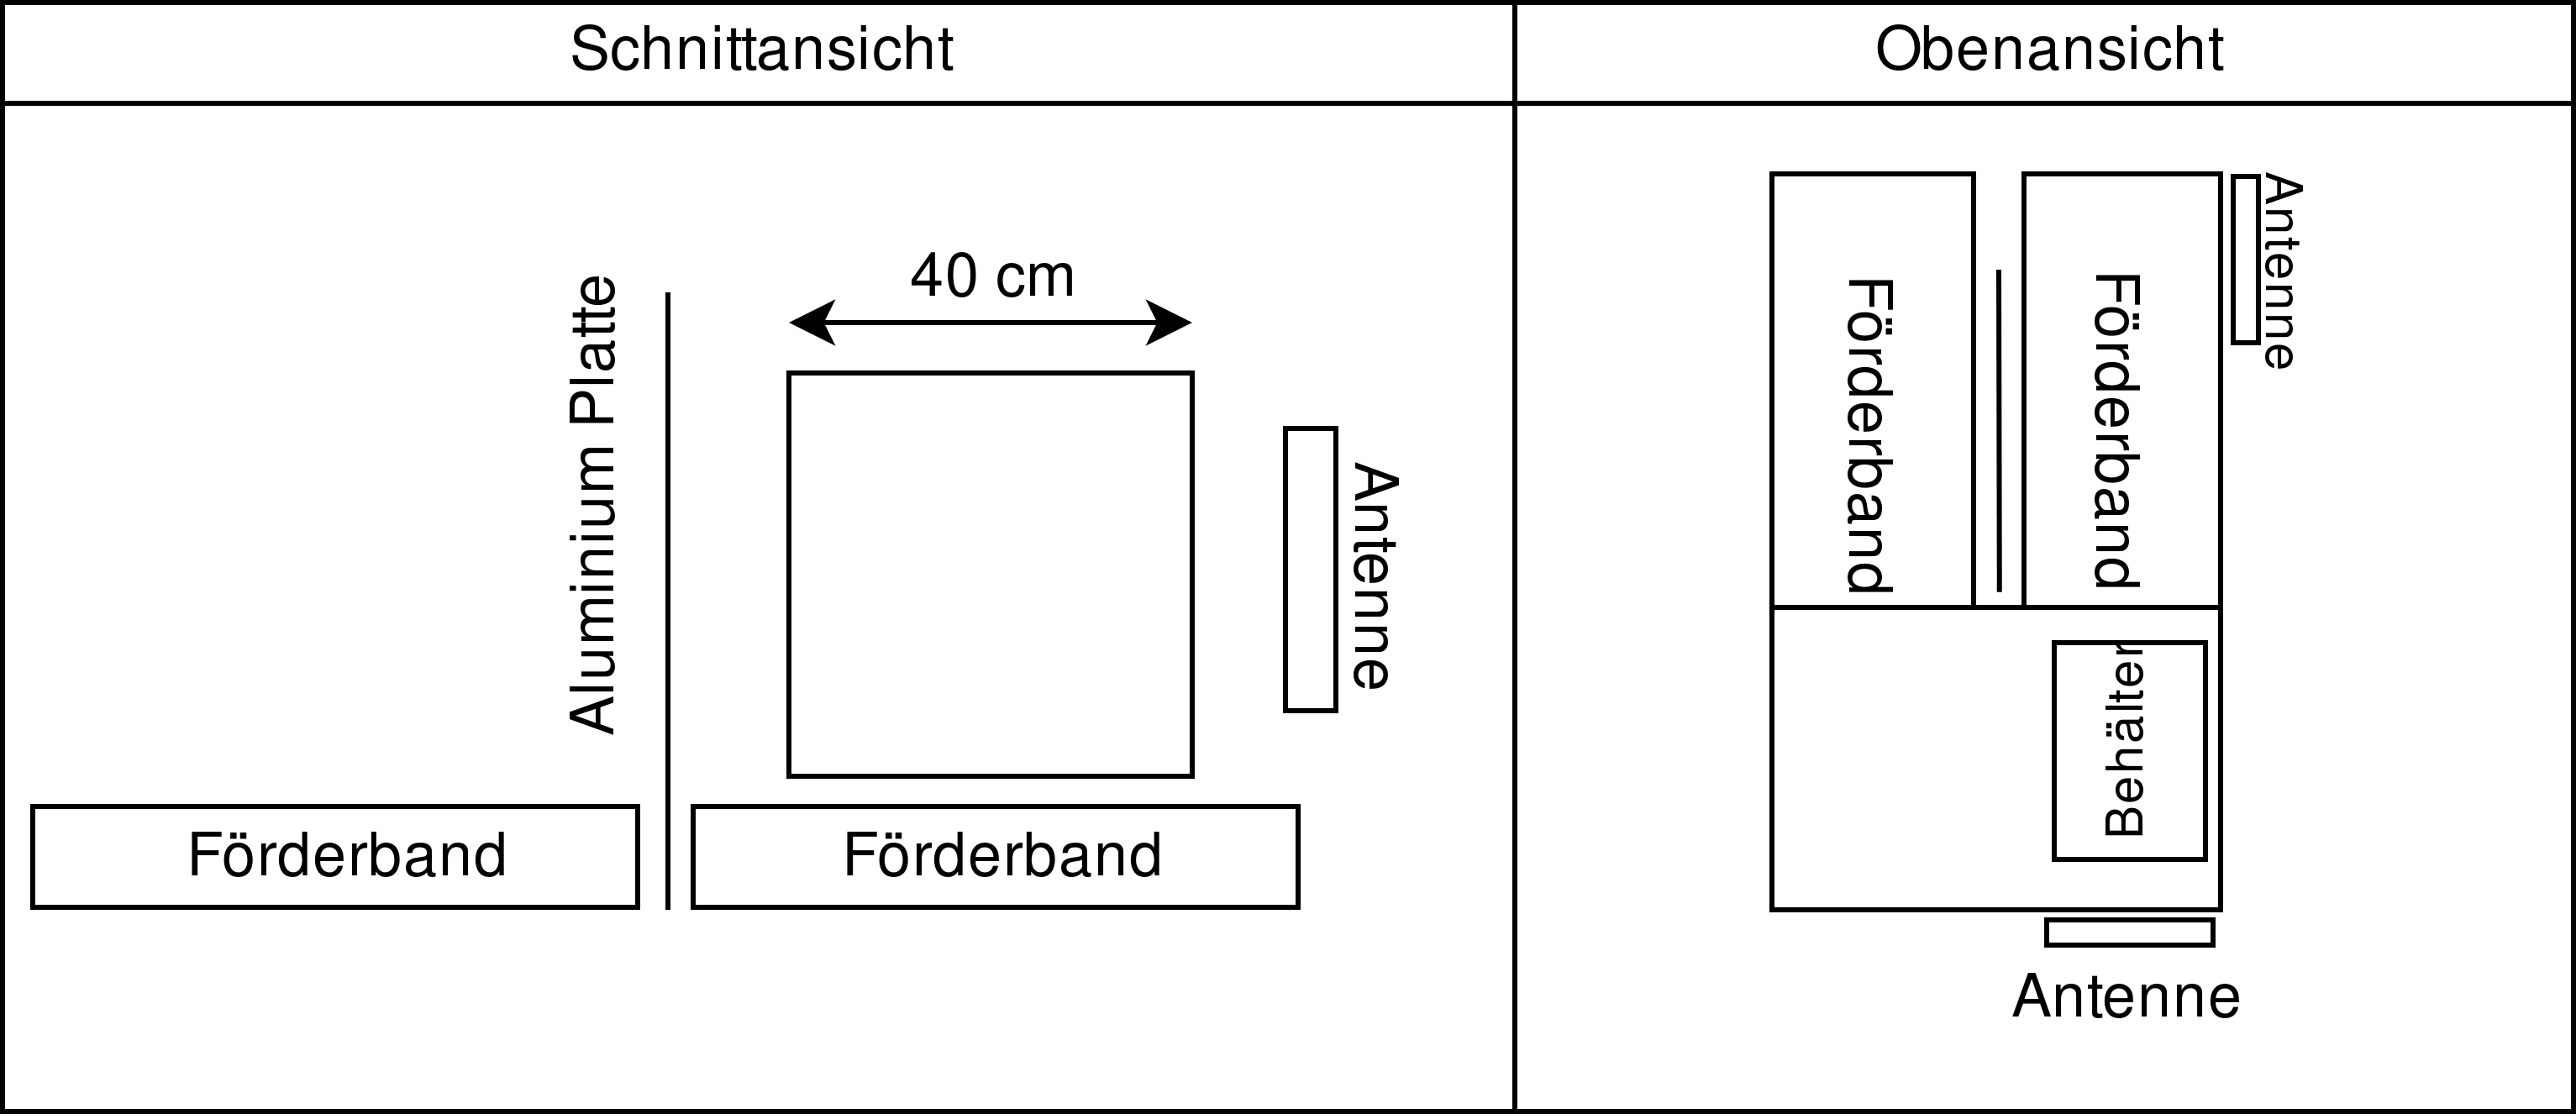
\includegraphics[keepaspectratio,width=\textwidth]{Position_Antennen}
	\caption{Positionierung einer Antenne über Förderband}
	\label{fig:PosAntennen}
\end{figure}

\begin{figure}[htb]
	\centering
	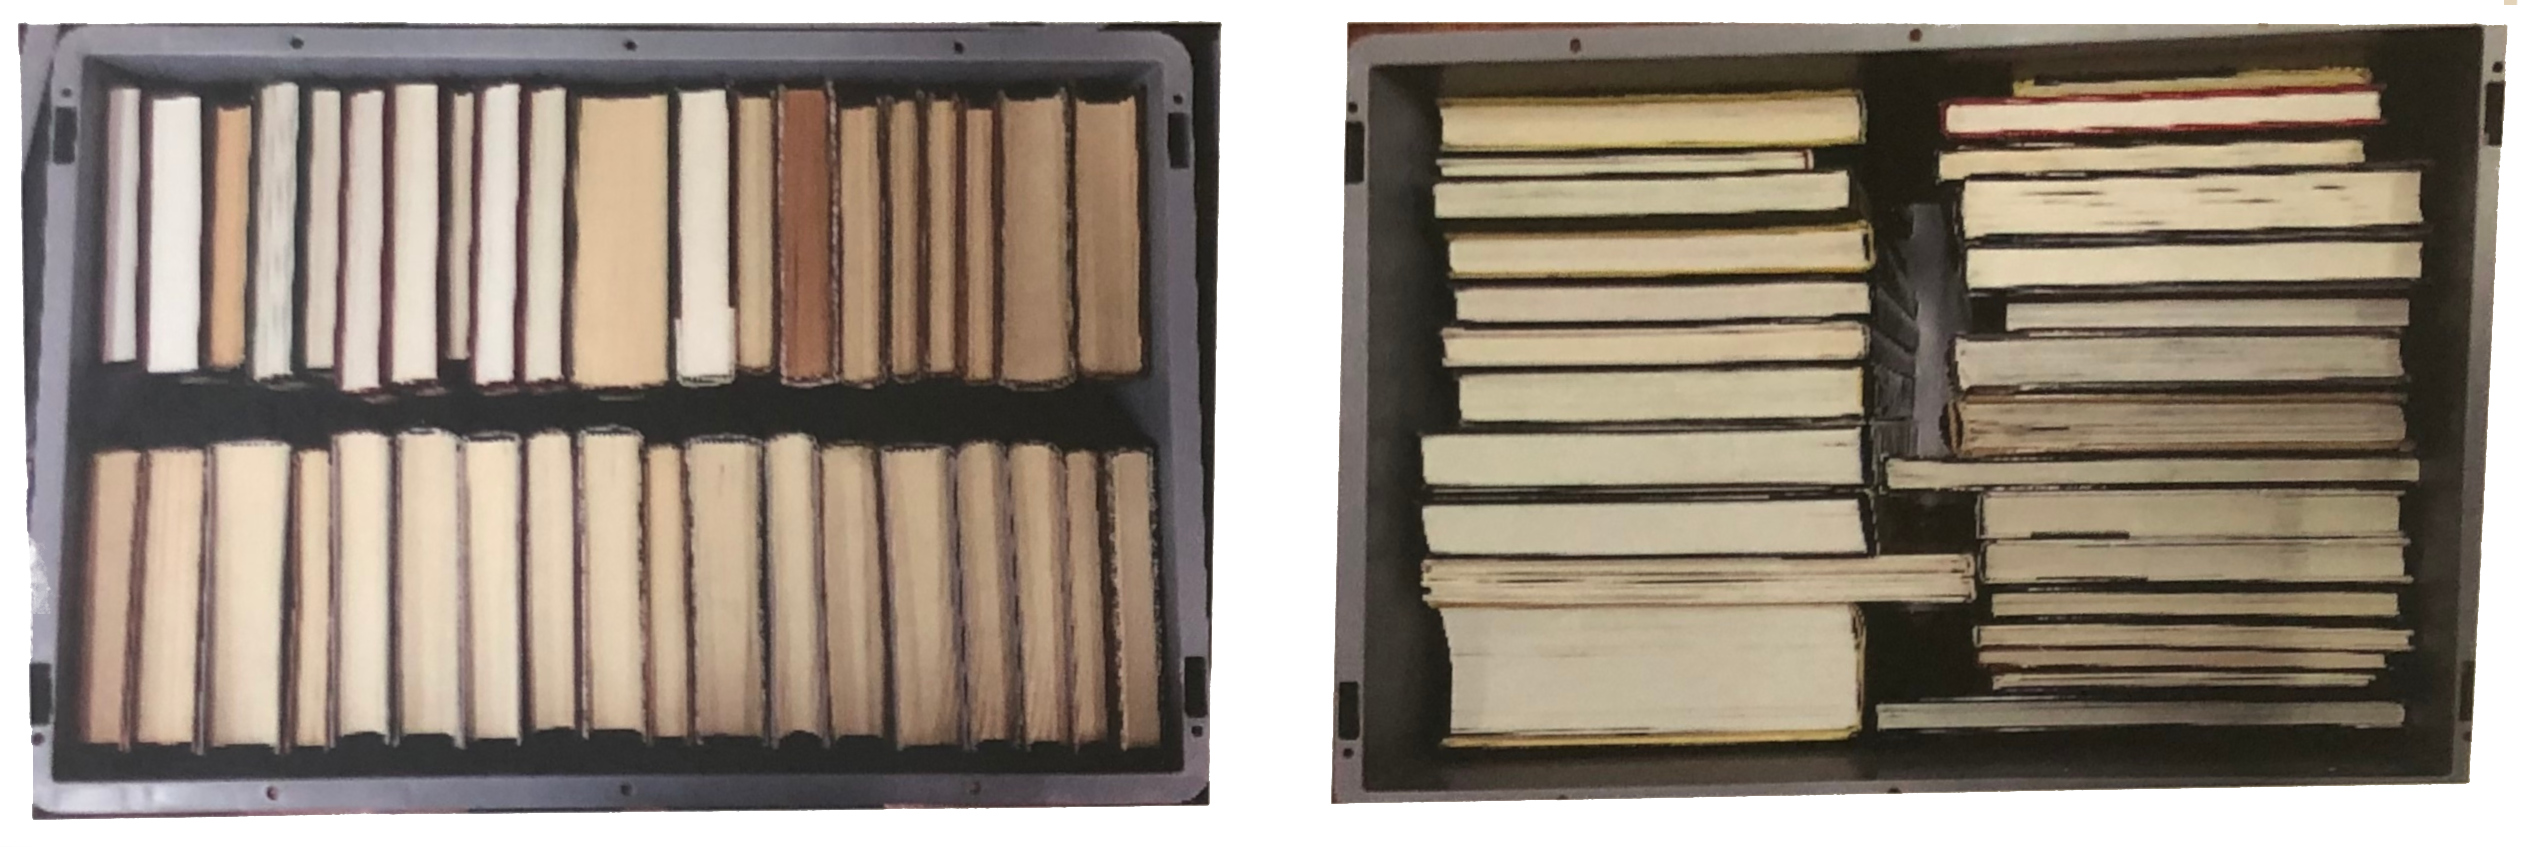
\includegraphics[keepaspectratio,width=\textwidth]{Lagerung_Exemplare}
	\caption{Arten wie die Exemplare in Behältern gelagert werden}
	\label{fig:LagExemplare}
\end{figure}

\subsection{Identifikation des Behälters}

\subsubsection{Barcodeleser}
An jedem Behälter ist ein Barcode aufgeklebt (auf beiden Seiten jeweils an der richtigen Stelle, sodass die Position durch eine Drehung überführt werden kann). Durch Auslesen dieses Strichcodes ist eine Eindeutige Identifikation des Behälters möglich.
\begin{itemize}
	\pro Behälter eindeutig identifiziert
	\pro Keine Abhängigkeiten
	\con Position muss stimmen, dass Barcode gelesen werden kann
\end{itemize}

\subsubsection{Bestimmung über die Mehrheit der Tags}
Falls man mehrere Tags identifiziert hat und weiss zu welchen Behältern diese gehören, kann man den nicht zum gleichen Behälter gehörenden Tag identifizieren.
\begin{itemize}
	\pro Positionsunabhängig
	\con Aktuelle Informationen über Tag und Behälter nötig (Schnittstelle Datenbank)
	\con Mindestens drei Tags müssen identifiziert worden sein
\end{itemize}

\subsection{Massnahmen nach Erkennungsprozess}

\subsubsection{Aussortierung des Behälters}
Es wäre vorstellbar, dass man den Behälter, nach einer Identifikation des Inhalts und Erkennen eines falschen Exemplars, aussortiert.
\begin{itemize}
	\pro Früh im Prozess
	\pro Wenig menschliche Interaktion für Aussortierung nötig
	\con Schnittstelle zum Steuerungssystem des Förderbands nötig
\end{itemize}

\subsubsection{Audiovisuelles Signal}
Man könnte eine Warnung abspielen sobald ein fehlplatziertes Exemplar identifiziert worden ist (Sirene, Warnlampe).
\begin{itemize}
	\pro Früh im Prozess
	\pro Keine Abhängigkeiten
	\con menschliche Interaktion für Aussortierung nötig
\end{itemize}

\subsubsection{Berichterstattung}
Man könnte, sobald ein fehlplatziertes Exemplar erkannt wurde, ein Bericht an die zuständige Stelle schicken.
\begin{itemize}
	\pro Verfolgbarkeit
	\pro Keine Abhängigkeiten zu Steuersystem
	\con Behälter muss manuell wieder aus dem Lager geholt werden
	\con Schnittstelle zu Meldesoftware nötig
\end{itemize}

\newpage

\subsection{Morphologischer Kasten und Variantenbeschreibung}

\begin{figure}[h!]
	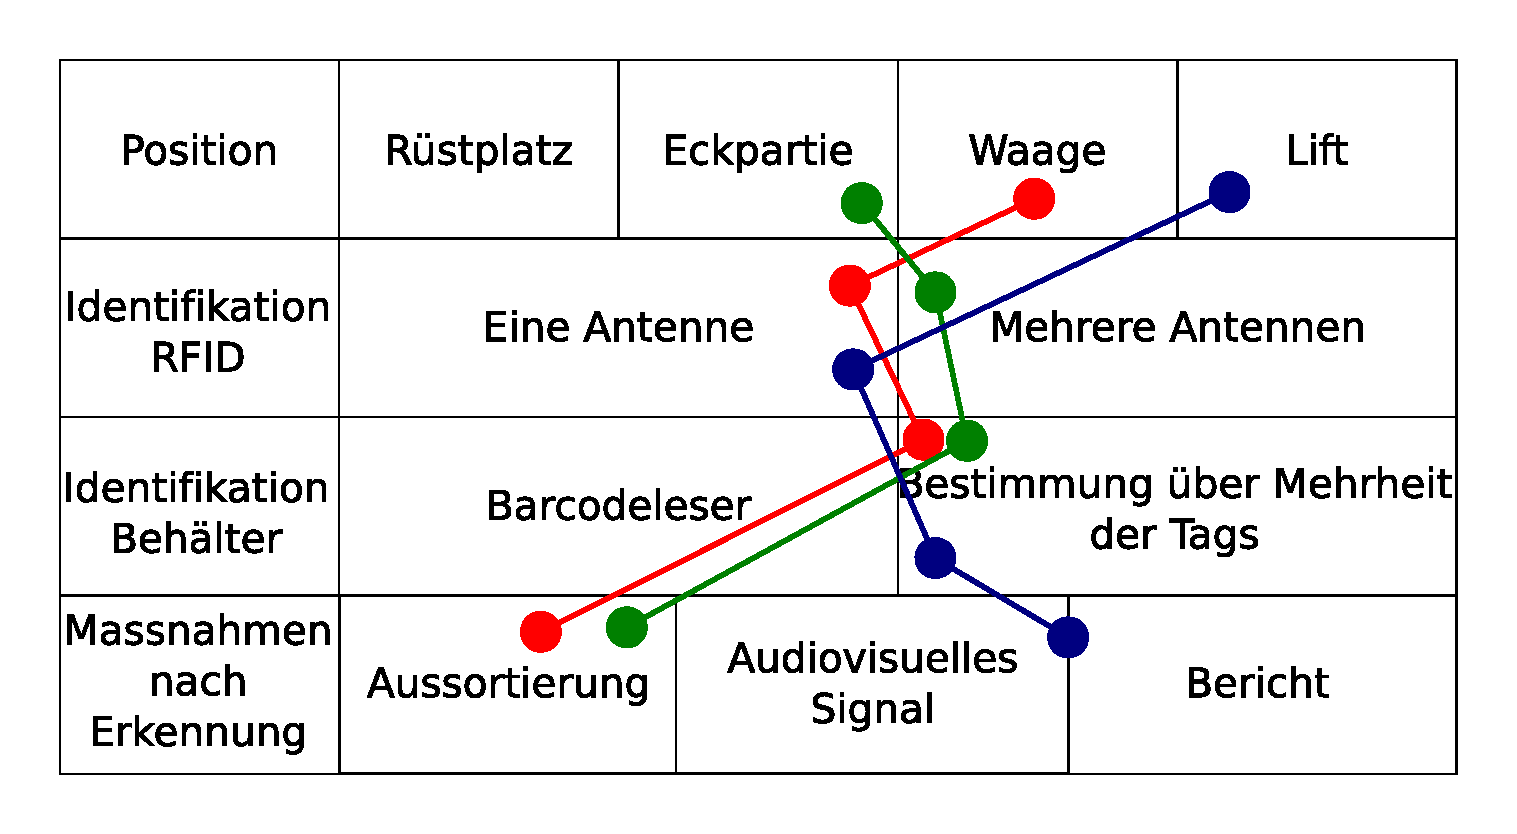
\includegraphics[keepaspectratio,width=\linewidth]{Morphologischer_Kasten}
	\caption{Die Varianten als Pfade dargestellt}
	\label{fig:MorphKasten}
\end{figure}

\subsubsection{Variante 1: Früherkennung und Aussortierung (Rot)}
In dieser Variante wurde Wert darauf gelegt, möglichst wenig Interferenzen zu haben, daher wurde sich für eine Antenne entschieden. Es soll über die Mehrheit der Tags der aktuelle Behälter bestimmt werden und falls Tags eines anderen Behälters gefunden wurde, der Behälter nicht eingelagert, sondern aussortiert werden (sprich ein Steuerungssignal an das Förderband gegeben werden). Der Ort wurde ausgewählt, da der Behälter dort eine kurze Pause einlegt. Diese Variante hängt stark davon ab wie schnell und fehlerfrei Tags ausgelesen werden können und ob eine Schnittstelle zur Steuersoftware existiert die wir nutzen können.

\subsubsection{Variante 2: Weitflächige Erkennung und Aussortierung (Grün)}
Es soll durch mehrere Antennen eine grössere Abdeckung erreicht werden und so sichergestellt werden, dass alle Tags ausgelesen werden können. Auch bei dieser Variante soll der Behälter über die Mehrheit der Tags ausgelesen werden, und dieser, wenn nötig, aussortiert werden.

\subsubsection{Variante 3: Erkennung und Signalisierung (Blau)}
Bei dieser Variante soll der Leser bei der Warteposition vor der Einlagerung positioniert werden, da dort die Behälter ein paar Sekunden verbleiben. Danach sollen die erkannten Tags und der Behälter als Mitteilung an die Arbeitsstation geschickt werden (Mail, Middleware, Signallampe). Das mögliche Problem dieser Variante ist, dass zwei Behälter nebeneinander in der Warteposition sein können, und dadurch allenfalls Falschpositive generiert werden können.

\subsection{Wahl der Variante}

Das Projektteam empfiehlt Variante Zwei, da in den Versuchen die Wichtigkeit der Ausrichtung der Tags festgestellt wurden. Daher werden zwei Antennen verwendet und wie in Abbildung \ref{fig:PosAntennen} dargestellt, damit die zwei Varianten der Bücherlagerung (in Abbildung \ref{fig:LagExemplare} dargestellt) gelesen werden können. Die Aussortierung wird empfohlen, damit der Prozess voll autonom geschieht.

\subsubsection{Übersicht der Hardwarekomponenten}
Es sollen folgende Komponenten verwendet werden:
\begin{itemize}
	\item RFID Leser ID ISC.LR2500-A  (Feig)
	\item RFID Antennen ID ISC.ANT800/600 (Feig)
	\item RFID Antennenkabel ID ISC.ANT.C-A (Feig)
	\item Netzteil für Leser ID NET.24V-B (Feig)
	\item Netzkabel für Netzteil ID CAB.NET.24V-B-EU  (Feig)
	\item Minicomputer Raspberry PI 3 Model B + (Raspberry PI)
	\item USB-Kabel für Minicomputer Aukey CB-D11 (Aukey)
	\item Sandisk Extreme 128GB Class 10
	\item Schnittstelle zu Lagerverwaltungssystem
\end{itemize}

\section{Finanzierungsplan}

Als Berechnungsgrundlage wird ein Konzept mit einer Antenne und einer Steuerung über das Netzwerk gerechnet. Die Daten von Feig wurden von Euro auf CHF umgerechnet (Wechselkurs 1.14). Zudem sind dies die Demopreise für einen Prototyp.

\vspace{1em}

\begin{tabularx}{\textwidth}{|r|X|r|r|}
	\hline 
	\textbf{Menge} & \textbf{Produkt} & \textbf{Kosten(CHF)} & \textbf{Kosten gesamt(CHF)} \\
	\hline 
	1 & RFID Reader ID ISC.LR2500-A (Feig) & 1'200 & 1'200 \\ 
	\hline 
	1 & RFID Antennen ID ISC.ANT800/600 (Feig)& 760 & 760 \\
	\hline
	1 & RFID Antennenkabel ID ISC.ANT.C-A (Feig) & 20 & 20 \\
	\hline
	1 & Netzteil ID NET.24V-B (Feig) & 30 & 30 \\
	\hline
	1 & Netzkabel ID CAB.NET.24V-B-EU (Feig) & 4 & 4 \\
	\hline
	1 & Raspberry Pi 3 Model B+ (pi-shop.ch)& 39 & 39 \\
	\hline
	1 & Sandisk Extreme 128GB Class 10 (digitec.ch)& 45 & 45 \\
	\hline
	& & & \textbf{2098} \\
	\hline
\end{tabularx} 


\chapter{Validation der Konzepte}

\section{Unbekannte im Bereich der Technischen Möglichkeiten}
Beide beschriebenen Konzepte setzten spezifische technische Möglichkeiten voraus, damit diese umgesetzt werden können. Für die Validation dieser technischen Möglichkeiten wurden verschiedene Versuche erstellt, welche mit einem zur Verfügung stehenden RFID Lesegerät durchgeführt werden sollen.

Für das Konzept zur Auffindung eines deplatzierten Exemplars im Hochregallager galt es folgende technische Möglichkeiten abzuklären:

\begin{itemize}
	\item Effektive Reichweite zum Auslesen eines Tags (min 97cm)
	\item Lesegeschwindigkeit eines Tags
	\item Lesbarkeit eines Tags bei Fahrt von 4m/s
	\item Seitliche Reichweite (Bei 60cm ca. 20cm)
	\item Ausrichtung des Tags
	\item Abschirmung und Störungen durch Metall, Bücher, WLAN sowie RAKO-Behälter
	\item Interferenz mehrerer Antennen
	\item Auslesen von gestapelten Tags
\end{itemize}

Für das Konzept zur Verhinderung der Einlagerung eines deplatzierten Exemplars im Hochregallager galt es folgende technische Möglichkeiten abzuklären:
\begin{itemize}
	\item Effektive Reichweite zum Auslesen eines Tags (min 54cm)
	\item Lesegeschwindigkeit Anzahl Tags (ca. 40Tags/s)
	\item Seitliche Reichweite (Bei 54cm ca. 20cm)
	\item Ausrichtung des Tags (bis zu 90\SIUnitSymbolDegree)
	\item Abschirmung und Störung durch Metall, Bücher, WLAN, Smartphone, Kreditkarten oder Stromquellen
	\item Interferenz mehrerer Antennen
	\item Auslesen von gestapelten Tags
\end{itemize}

Aus diesen abzuklärenden technischen Möglichkeiten wurden schliesslich folgende Versuche definiert, welche mit einem RFID Leser durchgeführt werden sollten:
\begin{enumerate}
	\item Effektive Reichweite gerade
	\item Lesegeschwindigkeit Bulk Reading
	\item Seitliche Reichweite
	\item Ausrichtung des Tags
	\item Abschirmung durch Gegenstände (Metall, Bücher, RAKO-Behälter)
	\item Interferenz mehrerer Antennen
	\item Auslesen bewegende Box
	\item Störung durch WLAN
	\item Störung durch Smartphone
	\item Störung durch Kreditkarte
	\item Störung durch Stromquellen
	\item Auslesen von gestapelten Tags
\end{enumerate}

Die genaue Versuchsanordnung ist im Anhang \ref{app:ch:versuche} zu finden.

\section{Vorgehen zur Abklärung der Technischen Möglichkeiten}

Durch das knappe Budget, welches dem Team zur Verfügung stand, konnte für die Hardwarebeschaffung kein inländischer Vertreiber verwendet werden. Es wurde schliesslich der chinesische Hardwarehersteller Hyintech für die Beschaffung der Hardware ausgewählt. Dabei wurde auf folgende Komponenten gesetzt:

\begin{itemize}
	\item HYH1W2T (RFID Lesegerät)
	\item 2x HYP3242 (RFID Antennen)
\end{itemize}

Die genauen Spezifikationen der Hardware können im Anhang \ref{app:ch:hardwarespez} gefunden werden.

Da sich zudem keine weiteren Hersteller für eine Leihgabe bereiterklärten, können alle folgenden Aussagen nur für die oben gelistete Hardware gemacht werden.

Für die Durchführung der Versuche wurden die Antennen auf einer hölzernen Vorrichtung befestigt, anschliessend wurde das Tag an einer weiteren Vorrichtung befestigt und in einer definierten Position gemäss den Versuchsbeschreibungen platziert und versucht auszulesen (siehe Abbildungen \ref{fig:versuchsaufbauten} a und b).

\begin{figure}[htb]
	\begin{subfigure}{.5\linewidth}
		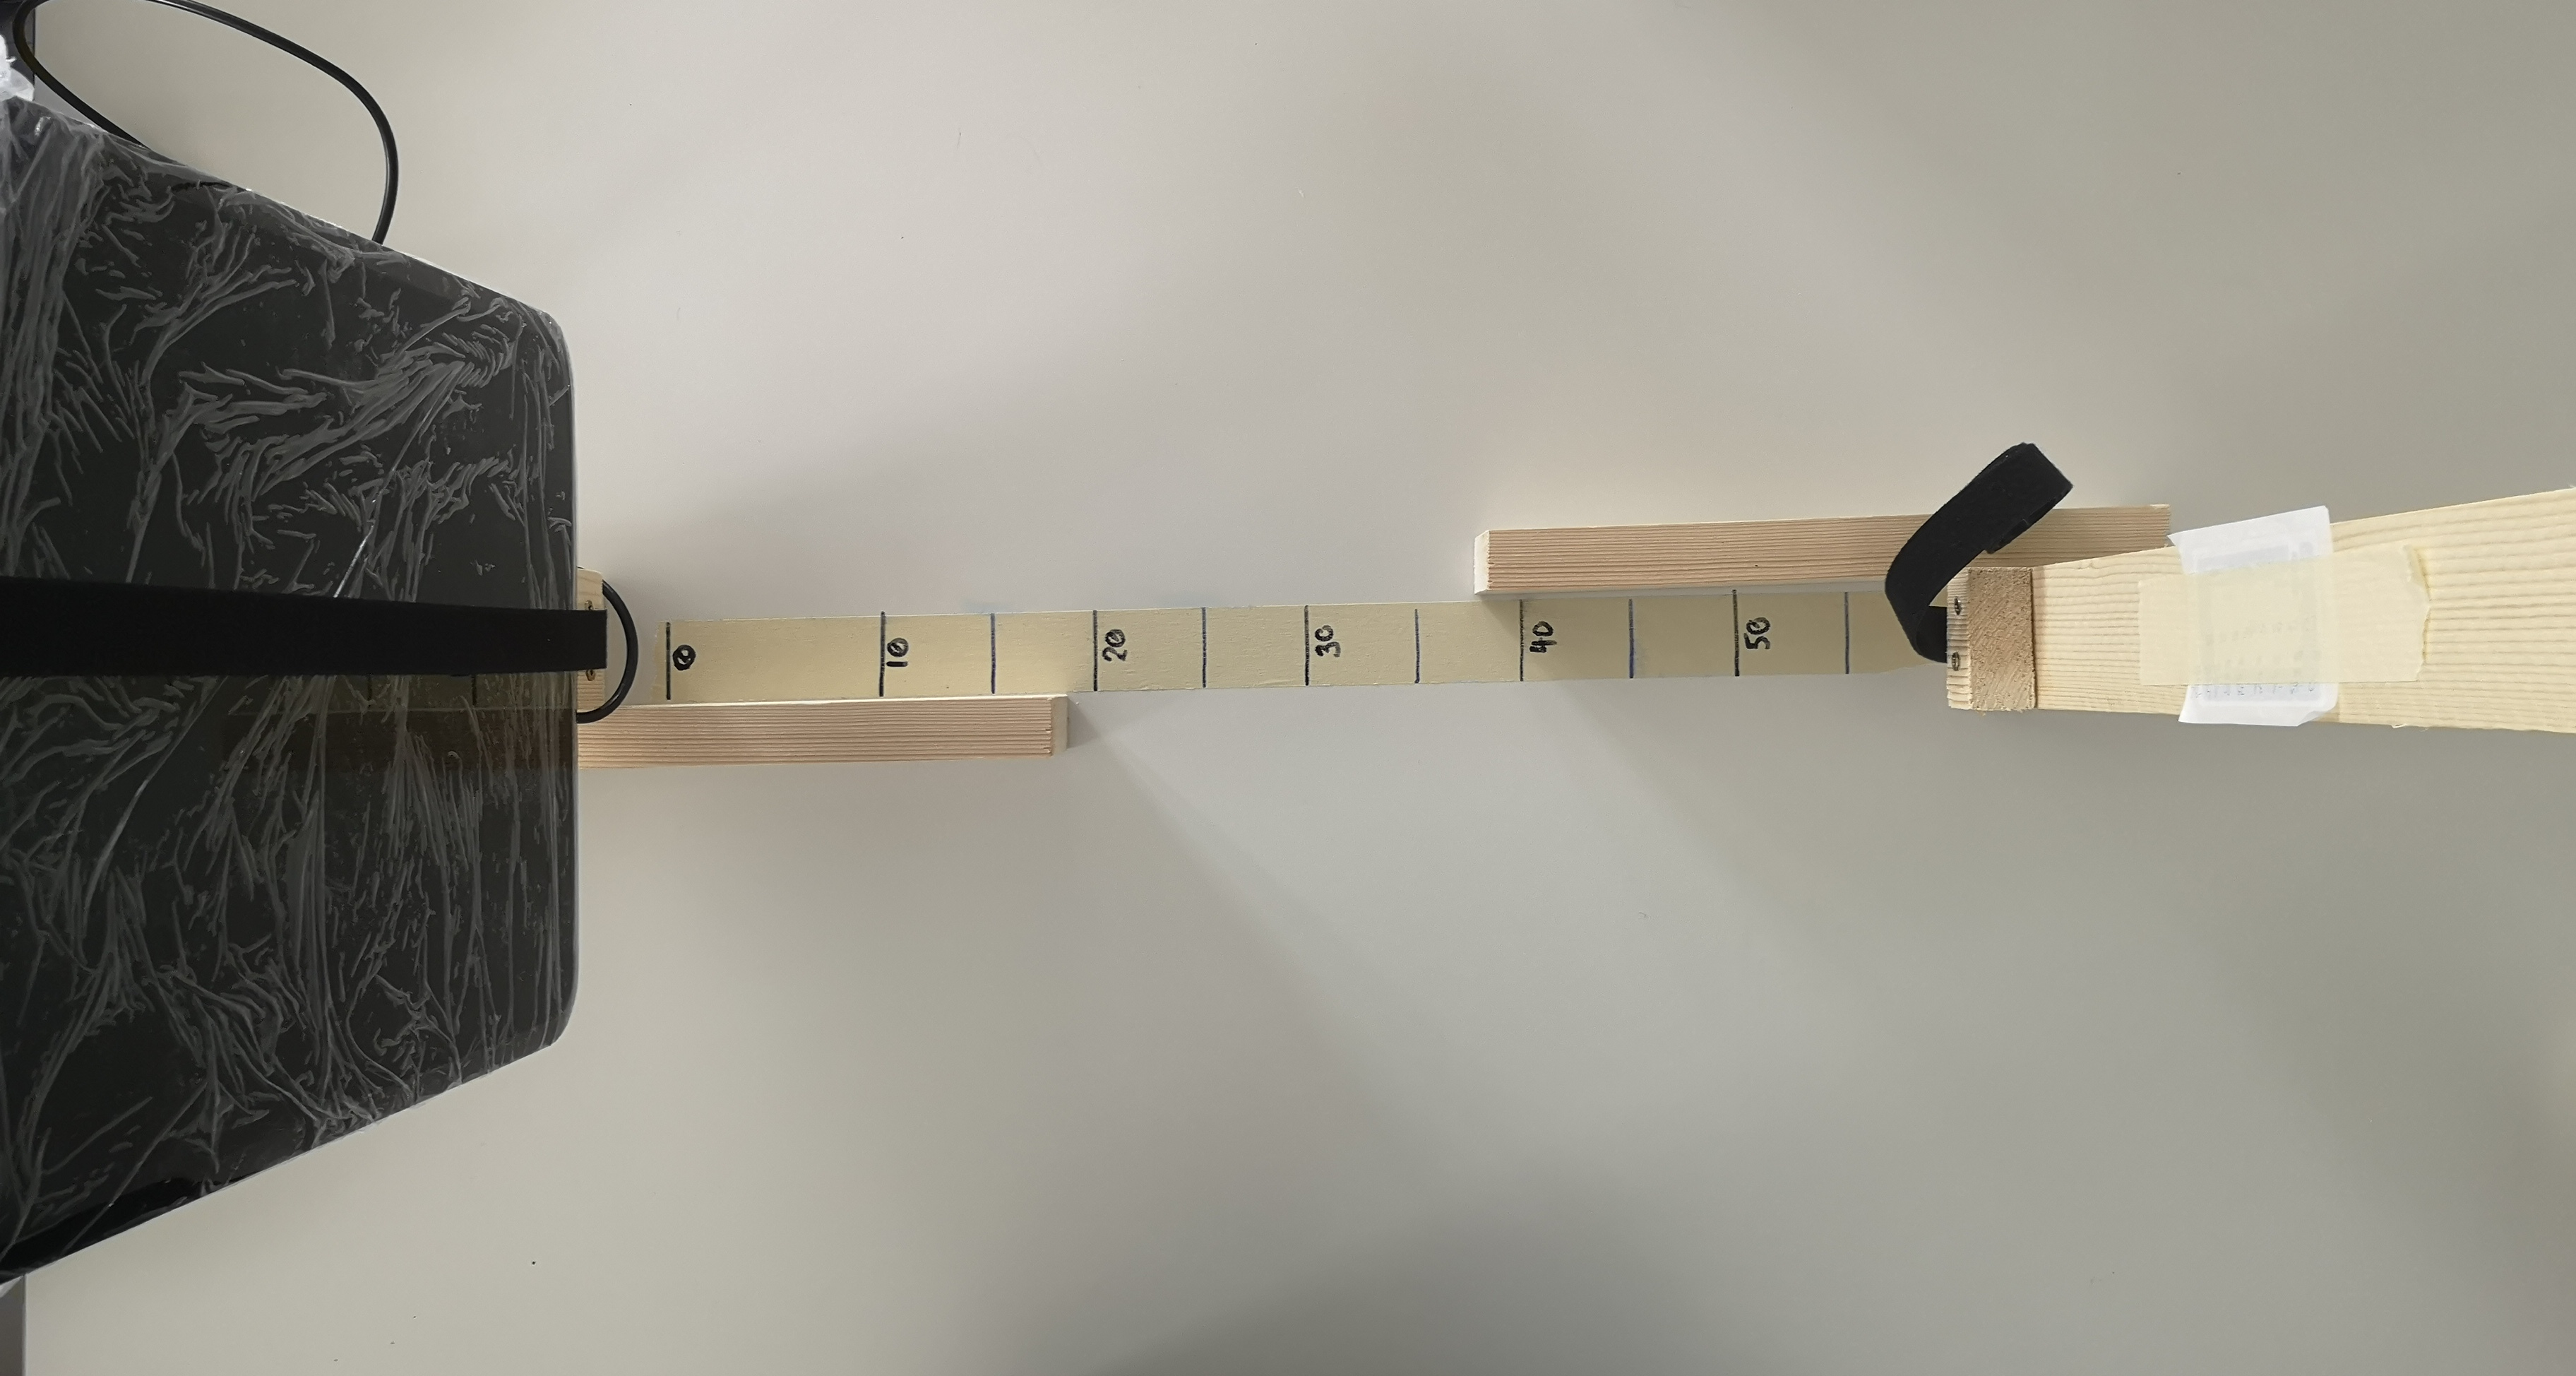
\includegraphics[keepaspectratio,height=4cm]{Versuch1MaximaleDistanz}
		\caption{Versuches Nummer 1 mit einem Abstand von 60cm}
		\label{fig:versuchaufbaunmr1}
	\end{subfigure}\hfill%
	\begin{subfigure}{.35\linewidth}
		\centering
		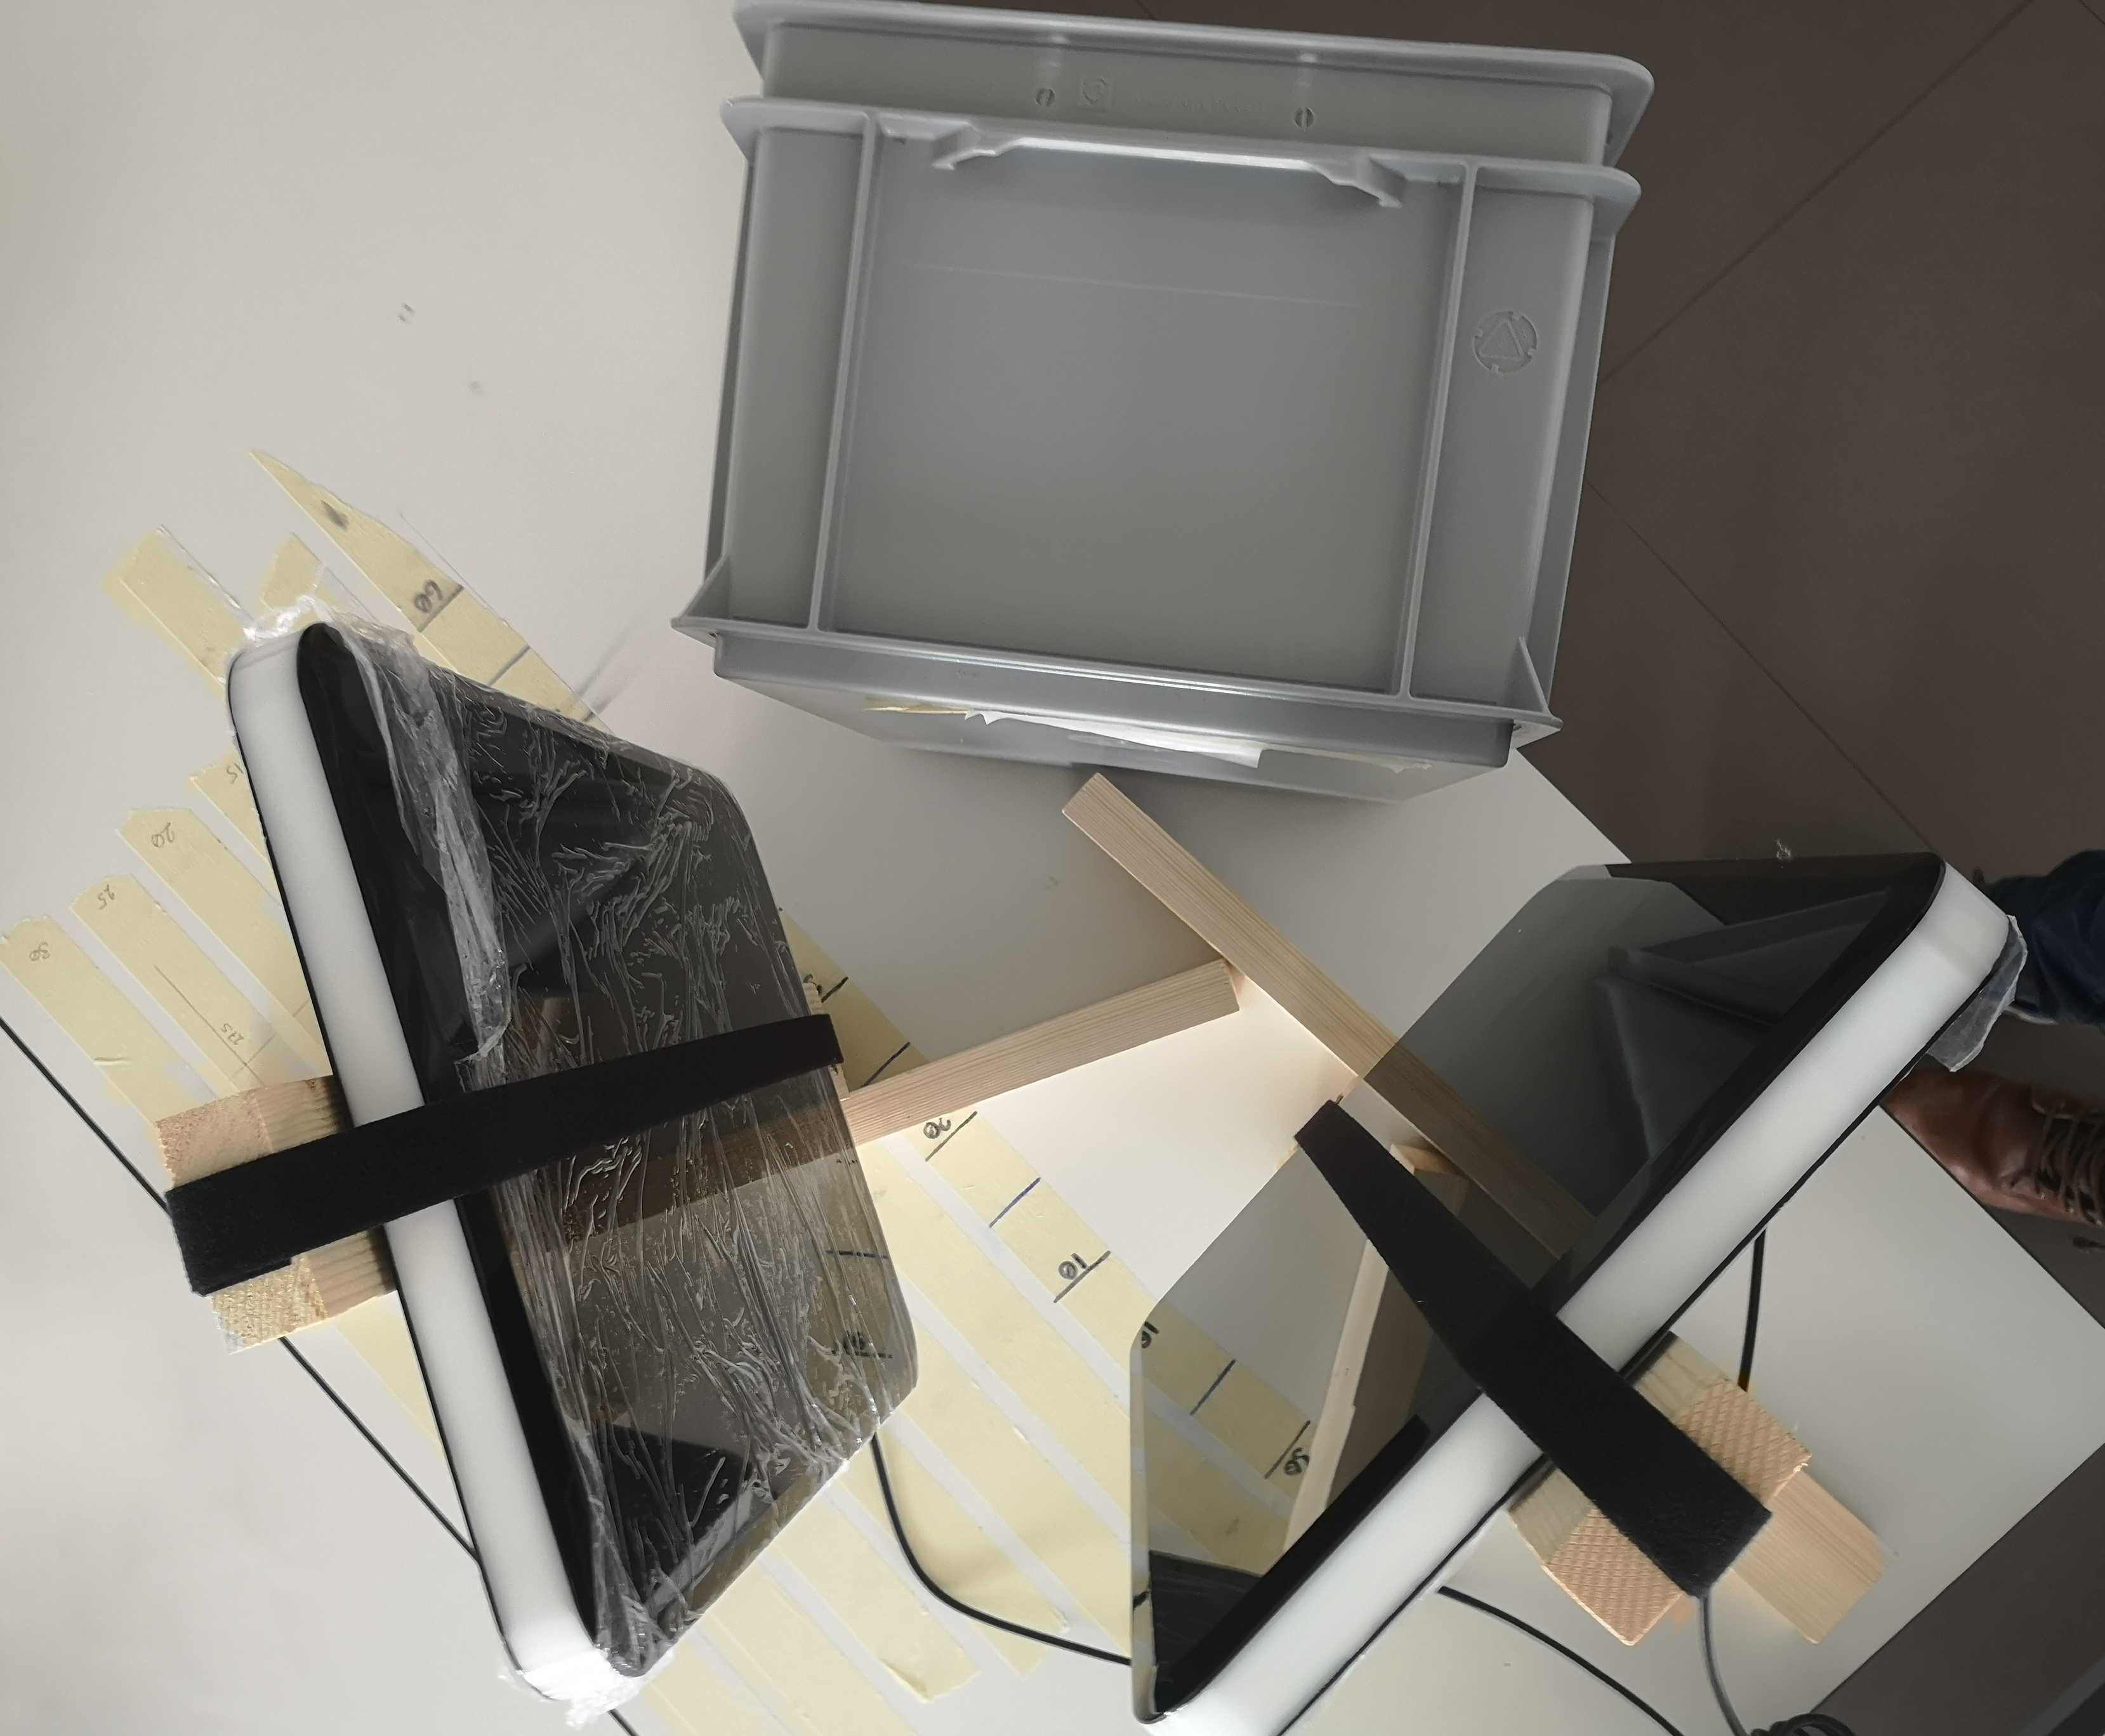
\includegraphics[keepaspectratio,height=4cm]{TestInterferenzAntennen}
		\caption{Versuch Nummer 7 mit einem Winkel von 60\SIUnitSymbolDegree}
		\label{fig:versuchaufbaunmr7}
	\end{subfigure}
	\caption{Zwei Versuchsaufbauten}
	\label{fig:versuchsaufbauten}
\end{figure}


\subsection{Software}
Da für viele Versuche eine genaue Messung eine wichtige Rolle spielt, wurde eine eigene Applikation geschrieben, welche für die Protokollierung der Resultate verantwortlich ist.

Bei der Implementierung der Software wurde darauf geachtet, dass die Kommunikation mit der Hardware bereits soweit abstrahiert wird, dass diese Komponente bei der Implementation eines Prototyps oder MVP wiederverwendet werden kann.

Der vereinfachte Aufbau der Applikation ist in Abbildung \ref{fig:test_applikation_aufbau} dargestellt. Für die Kommunikation mit der Hardware wurde zuerst angenommen, dass diese über RS232 stattfindet und diese Schnittstelle vom Hersteller dokumentiert sei. Es stellte sich jedoch heraus, dass Hyientech lediglich eine DLL zur Verfügung stellt, welche selber über die RS232 die Verbindung aufbaut und mit dem Gerät kommuniziert. Die genauen Spezifikationen zu dieser DLL können im Anhang \ref{app:ch:dllspezifikation} gefunden werden.

\begin{figure}[htb]
	\centering
	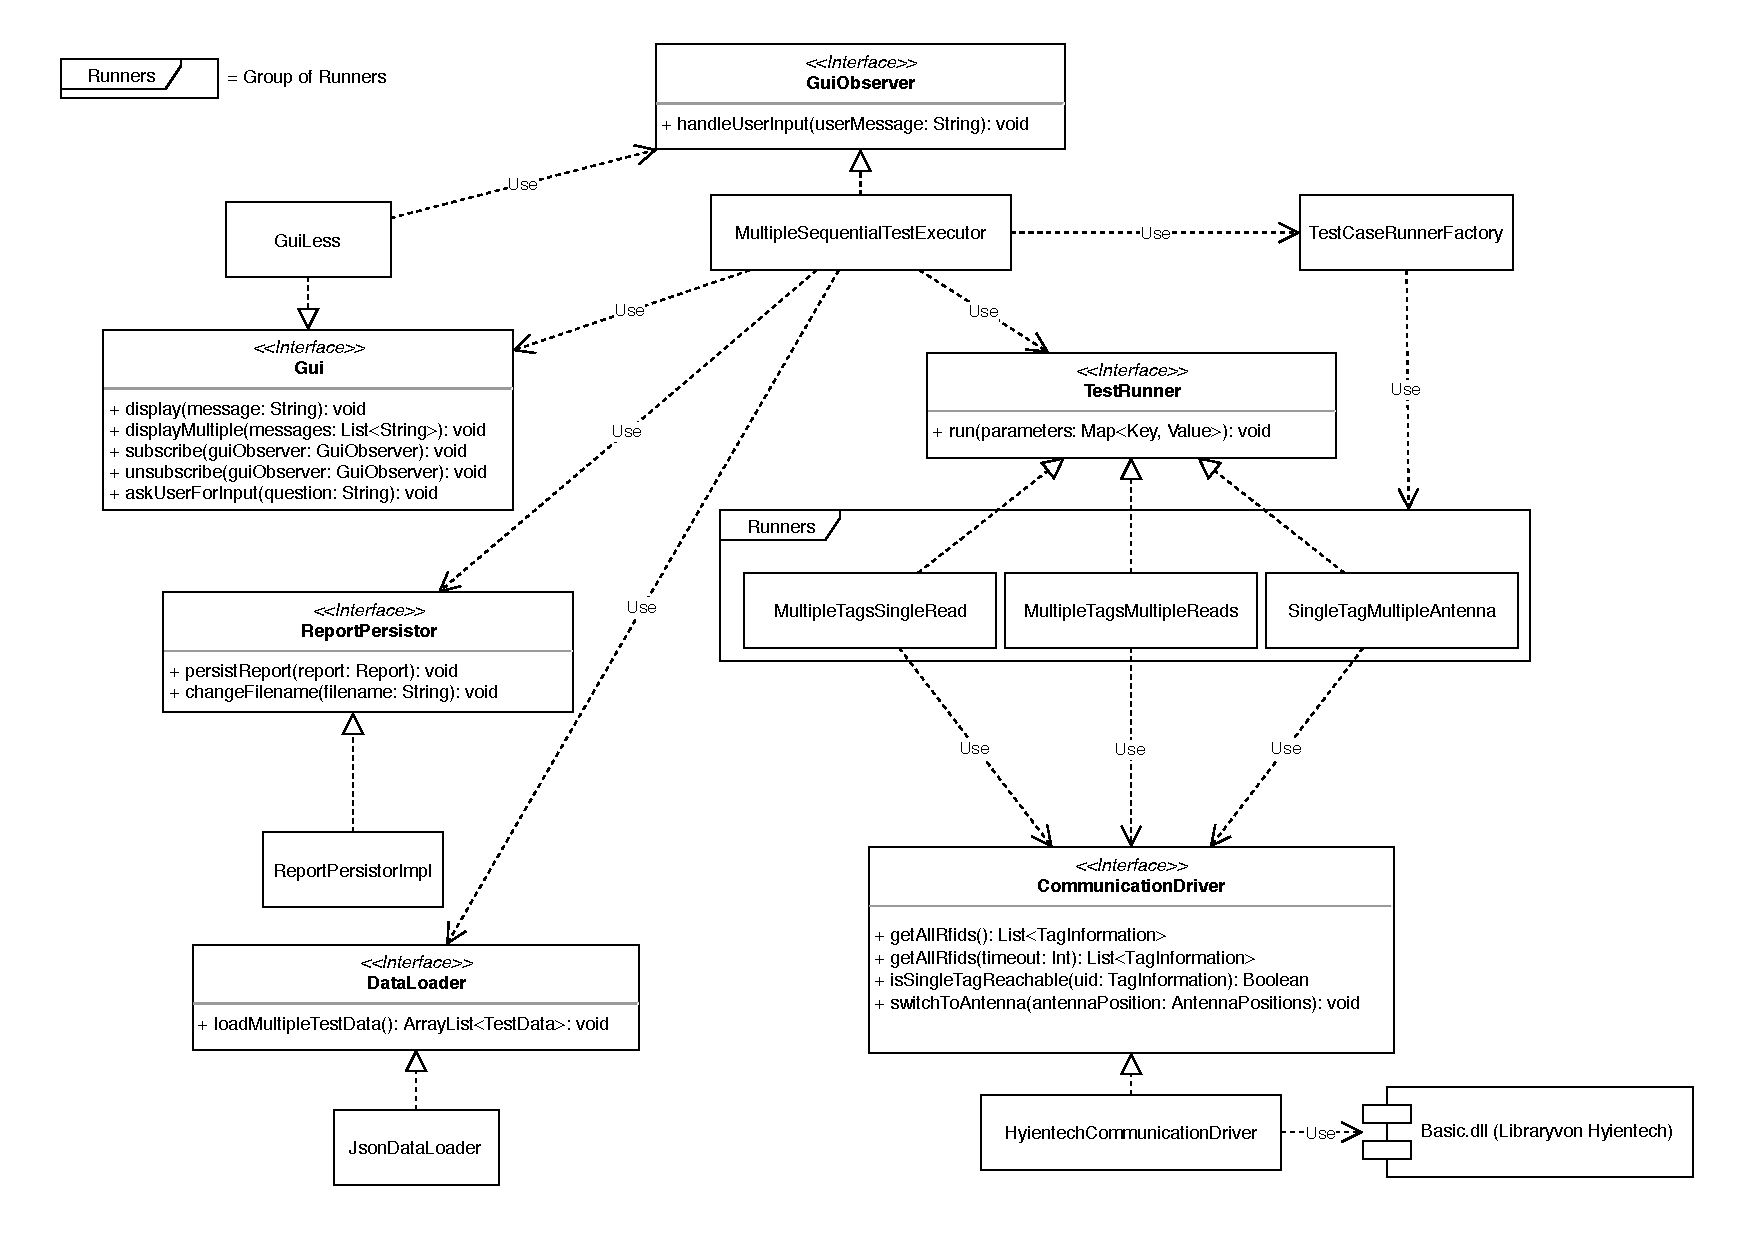
\includegraphics[keepaspectratio,width=\linewidth]{TestApplikation}
	\caption{Vereinfachte Darstellung der Testapplikation ohne POJOs}
	\label{fig:test_applikation_aufbau}
\end{figure}
 
\section{Erkenntnisse der Technischen Möglichkeiten}
Es konnte festgestellt werden, dass die Reichweite der Antenne den Herstellerangaben entsprechen, sofern der Tag parallel zur Antenne ausgerichtet ist. Ist der Tag in einer Achse gedreht, so funktioniert die Auslesung ab einem Auslenkungswinkel von 60\SIUnitSymbolDegree\ nicht mehr. Weiter konnte die Lesegeschwindigkeit für 15 TagIDs ermittelt werden, welche bei rund 350ms liegt. Es wurde daher geschlussfolgert, dass es möglich ist 40 TagIDs pro Sekunde auszulesen.
Bei einer optimalen Ausrichtung konnte die seitliche Reichweite bei einer Distanz von 50cm zur Antenne auf 25cm, respektive bei 60cm zur Antenne auf 12.5cm ermittelt werden. Wie schon beschrieben, können maximal ausgelenkte Tags (90\SIUnitSymbolDegree) in der Flucht der Antenne nicht ausgelesen werden. In den Versuchen wurde ermittelt, dass der Tag, bis zu einer Distanz von 30cm zur Antenne, gelesen werden kann, sofern sich dieser nicht direkt in der Flucht befindet (siehe Abbildung \ref{fig:Seitlich90}).

\begin{figure}[htb]
	\centering
	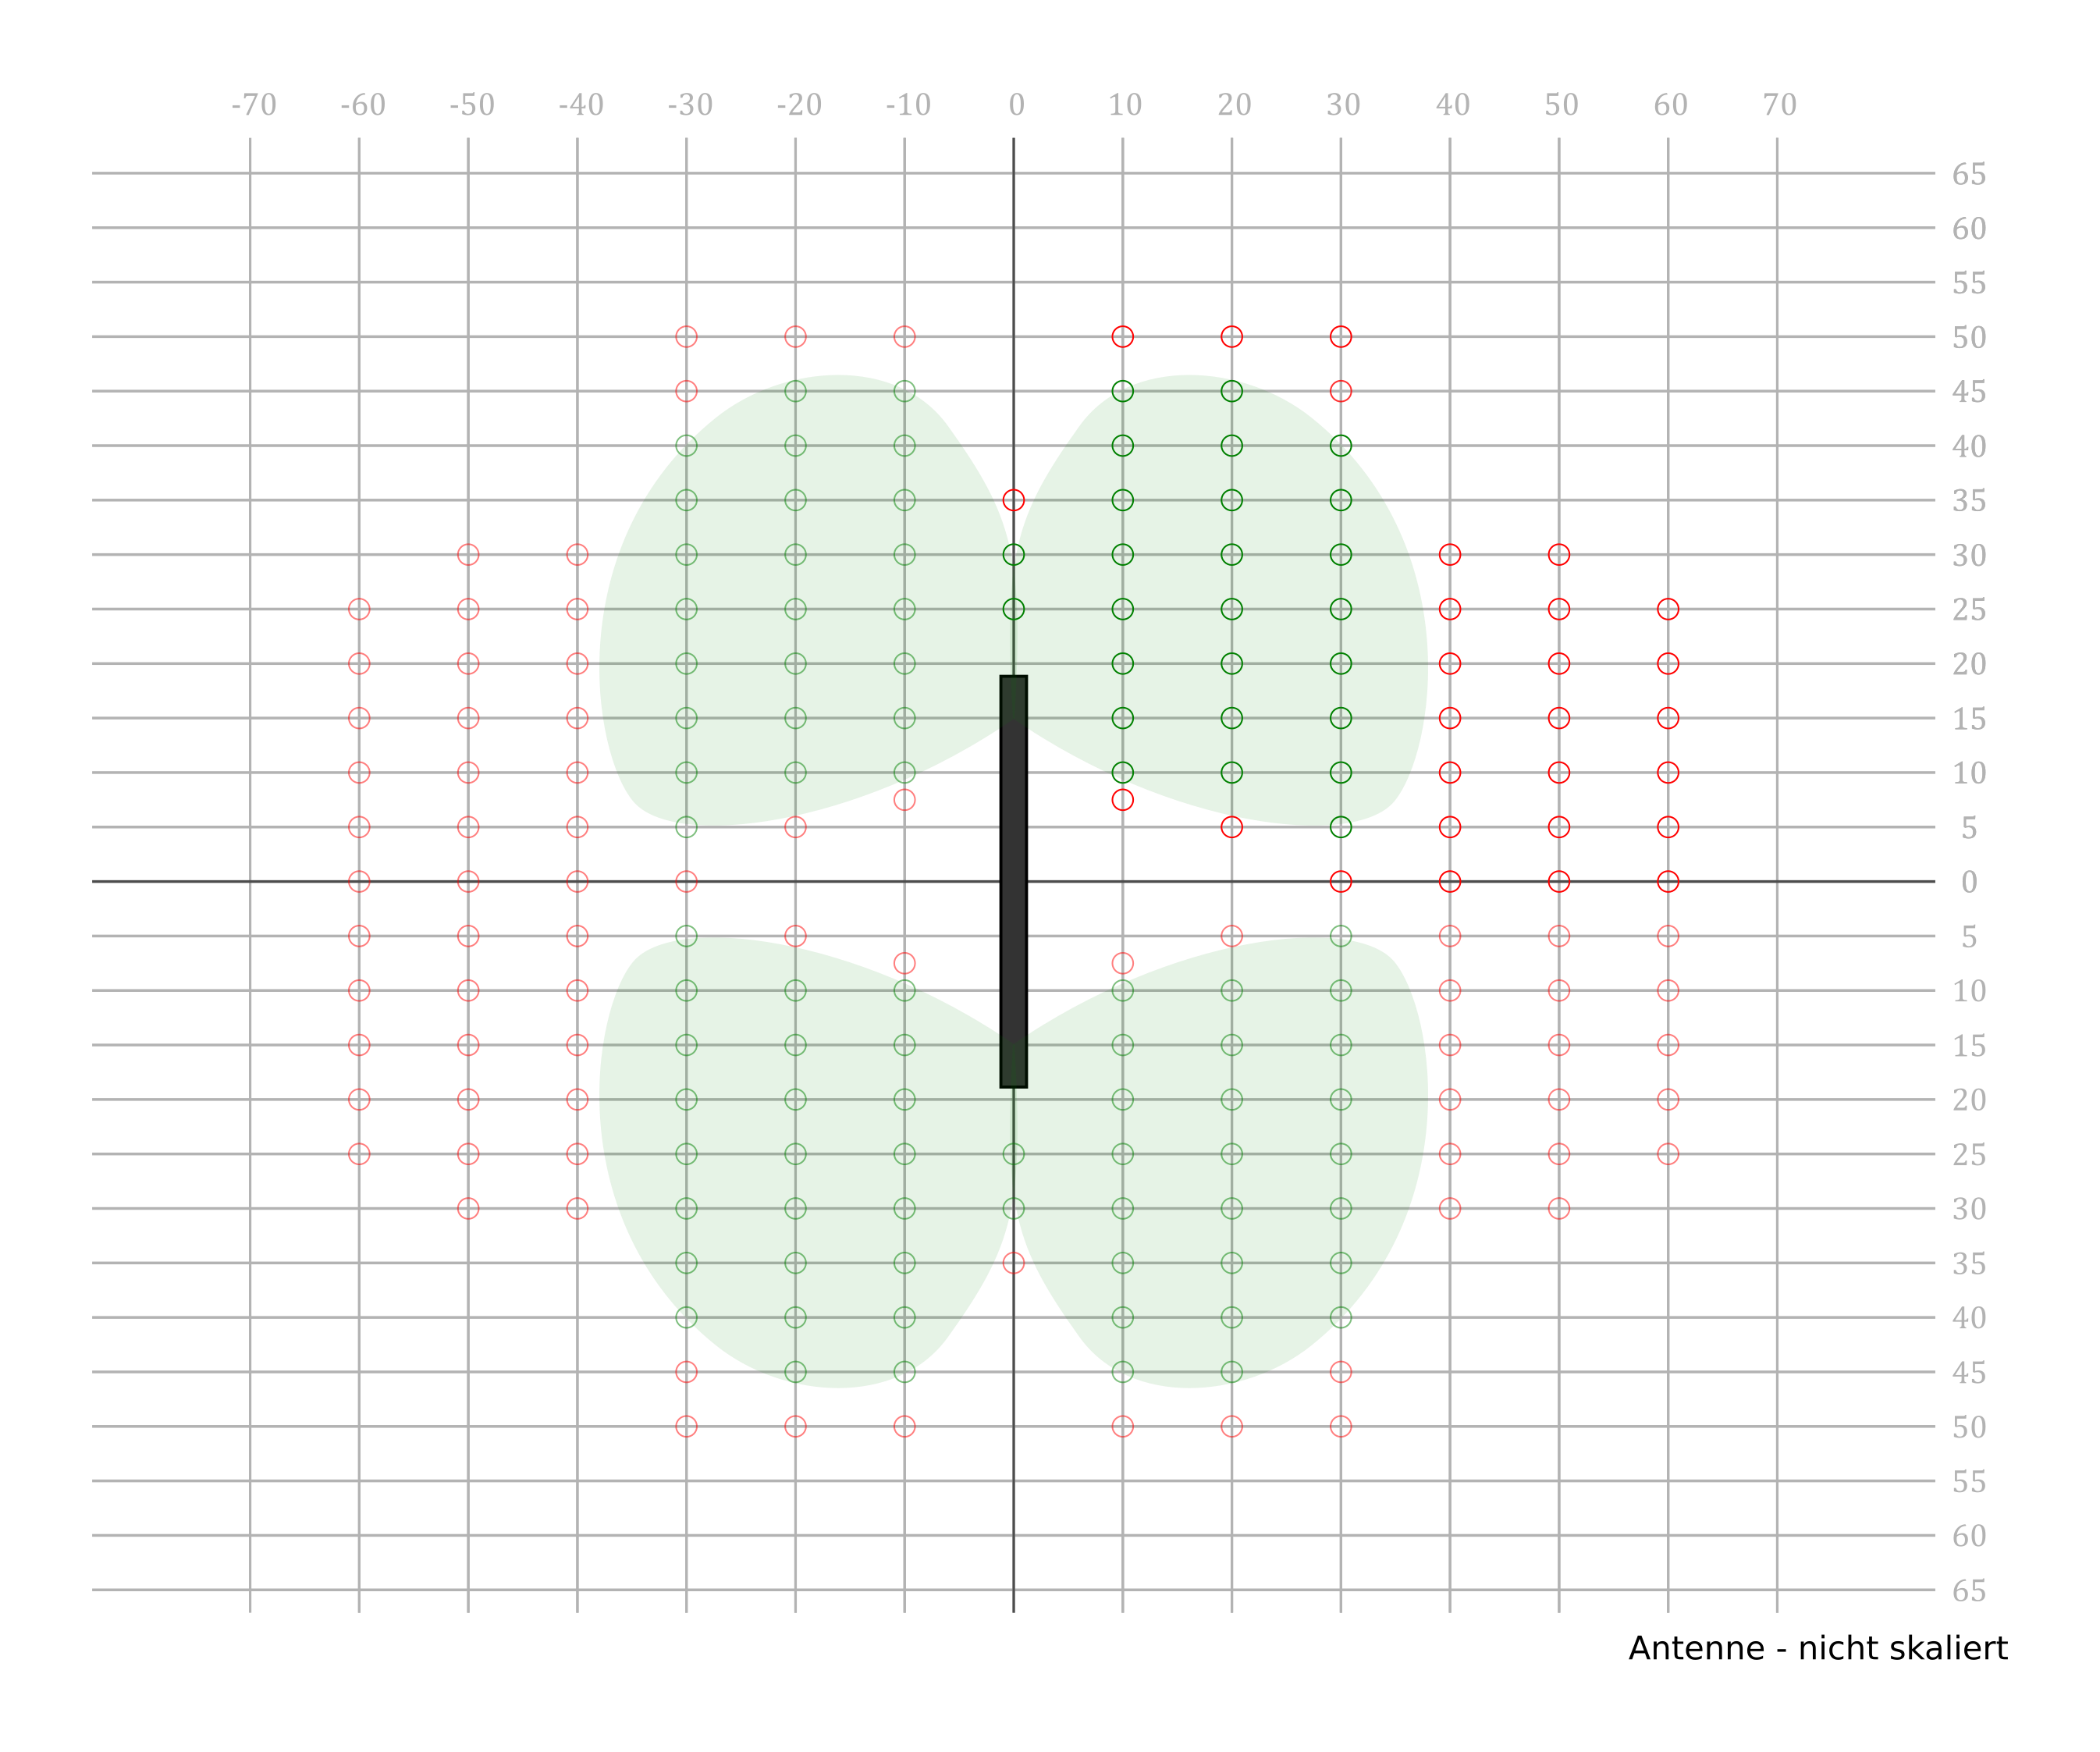
\includegraphics[keepaspectratio,height=7cm]{ResultateModell90}
	\caption{Ein Modell der Erreichbarkeit eines Tags mit 90\SIUnitSymbolDegree Auslenkung}
	\label{fig:Seitlich90}
\end{figure}

Weiter konnte in den Versuchen festgestellt werden, dass das Lesen durch ein Metall, sei dies Aluminium oder Stahl, unmöglich ist. Keiner der Tags hinter einer Metallplatte, im Minimum 0.75mm dick, konnte gelesen werden. Es konnte jedoch keine Abschirmung durch Bücher, Plastikbehälter, WLAN oder Hände festgestellt werden. Die Interferenz der Antennen konnte insofern nicht getestet werden, dass die Antennen nicht parallel betrieben werden konnten. Bei gestapelten Tags konnte eine starke Interferenz festgestellt werden. Um alle Tags erfolgreich auslesen zu können, muss ein Mindestabstand von 1.5cm in horizontaler und 3cm in vertikaler Richtung eingehalten werden.

\section{Fazit der Validation}
Das Konzept zur Auffindung eines deplatzierten Exemplares im Hochregallager musste nach den gewonnen Erkenntnissen verworfen werden und wurde daher für die Machbarkeitsstudie nicht beachtet. Die Problematik der Auslenkung führte zu einer Anpassung in der Positionierung der Antennen im Design des Konzepts zur Verhinderung eines Deplatzieren eines Exemplars vor Einlagerung in das Hochregallager, aber das Konzept wurde nach der Validiation der technischen Möglichkeiten immer noch als machbar eingestuft.